\documentclass{article}
\usepackage[UKenglish]{babel}
\usepackage[UKenglish]{isodate}
\usepackage{fullpage}
\usepackage{graphicx}
\usepackage{hyperref}
\usepackage{listings}
\usepackage{tikz-uml}

\title{Automated Benchmarking of Container Applications}
\author{Paulius Dilkas}

\begin{document}
\maketitle

%\begin{abstract}
%\end{abstract}

\section{Introduction}

% TODO:
% Motivation
% OpenShift, MiniShift
% Prometheus
% Flink
% Docker

\section{Architecture}

Two simple Dockerfiles were created. The first one is used for TaskManager and
JobManager pods and extends the original Flink Docker image by enabling
Prometheus support on port 9250. Prometheus can then query that port in order to
retrieve and record performance metrics.

The second Dockerfile extends the first one by adding a JAR file with Java code
for both the control server and the Flink app. This image also contains a custom
\texttt{ENTRYPOINT} that sends the Flink app to the JobManager (via port 8081)
as a background process, while executing the control server in the foreground.
This is the optimal arrangement of the two processes since the control server
always waits for the Flink app to finish in order to take its running time into
account when requesting data from Prometheus.

In both cases, one needs to change the permissions and group ownership of the
\texttt{/opt/flink} directory (to \texttt{775} and \texttt{root}, respectively)
so that the containers can be successfully executed by any user belonging to the
group \texttt{root}. Both images were put on Docker Hub, as this was the
simplest way to make them available to MiniShift.

A Docker Compose file was written with three services: Control,
JobManager, and TaskManager, establishing open ports as pictured in
Figure~\ref{fig:uml}). This file was then converted to OpenShift manifestos
using Kompose\footnote{\url{http://kompose.io/}}. The generated manifestos,
relevant network connections, and other dependencies are displayed in
Figure~\ref{fig:uml}.

Prometheus add-on for
MiniShift\footnote{\url{https://github.com/minishift/minishift-addons/tree/master/add-ons/prometheus}}
was modified to disable OAuth-based authentication by replacing
\texttt{-skip-auth-regex=\^{}/metrics} with \texttt{-skip-auth-regex=\^{}/}.
Furthermore, its configuration file was updated to set both scrape and
evaluation intervals to 1 second and the list of targets to JobManager and
TaskManager, both on port 9250.

Configuration Files component represents a ConfigMap created using the
\texttt{oc} command that contains two configuration files, \texttt{global.yaml}
and \texttt{components.yaml}. The former has the following...
% TODO: describe the config files

% TODO: finish explaining the diagram
% TODO: how do we start this (i.e., describe the Makefile)
\begin{figure}
  \centering
  \begin{tikzpicture}
    % components: first column
    \umlbasiccomponent[x=-6, y=3, fill=cyan!20]{Prometheus}
    \begin{umlcomponent}[fill=cyan!20]{Configuration Files}
      \umlbasiccomponent[x=-6, y=-2, fill=red!20]{Global}
      \umlbasiccomponent[x=-6, y=-4, fill=red!20]{Components}
    \end{umlcomponent}

    % components: second column
    \umlbasiccomponent[x=0, y=1]{Control Service}
    \begin{umlcomponent}{Control Pod}
      \umlbasiccomponent[x=0, y=-2, fill=red!20]{Control Server}
      \umlbasiccomponent[x=0, y=-4, fill=red!20]{Benchmarker}
    \end{umlcomponent}
    \umlbasiccomponent[x=0, y=-7]{Control Persistent Volume Claim}
    \umlbasiccomponent[x=0, y=-10]{Control Persistent Volume}

    % components: third column
    \umlbasiccomponent[x=6, y=3]{JobManager Service}
    \umlbasiccomponent[x=6, y=-1]{JobManager Pod}
    \umlbasiccomponent[x=6, y=-4]{TaskManager Service}
    \umlbasiccomponent[x=6, y=-8]{TaskManager Pod}

    % connections in second column
    \umlVHVassemblyconnector{Control Persistent Volume Claim}{Control Persistent Volume}
    \umlVHVassemblyconnector{Control Pod}{Control Persistent Volume Claim}
    \umlprovidedinterface[interface=998, with port, distance=2.5]{Control Server}
    \umlrequiredinterface[interface=998, with port]{Benchmarker}
    \umlHVassemblyconnector{Control Service}{Control Server-west-interface}
    \umlHVassemblyconnector{Control Service}{Benchmarker-east-interface}

    % connections between first and second columns
    \umlHVHassemblyconnector[interface={\space}, arm1=-2.3]{Benchmarker}{Global}
    \umlVHVassemblyconnector[interface={\space}]{Control Server}{Global}
    \umlVHVassemblyconnector[interface={\space}, arm1=-0.7]{Benchmarker}{Components}

    % Prometheus connections
    \umlHVHassemblyconnector[interface=HTTPS, arm1=-2, with port]{Control Server}{Prometheus}
    \umlassemblyconnector[interface=9250, arm1=1, with port]{Prometheus}{JobManager Service}
    \umlHVHassemblyconnector[interface=9250, arm1=8, with port]{Prometheus}{TaskManager Service}

    % column 3 connections
    \umlVHVassemblyconnector[interface={6123{,} 6124{,} 8081{,} 9250}, with port]{JobManager Pod}{JobManager Service}
    \umlVHVassemblyconnector[interface={6121{,} 6122{,} 9250}, with port]{TaskManager Pod}{TaskManager Service}
  \end{tikzpicture}
  \label{fig:uml}
  \caption{UML component diagram of the system, as deployed on MiniShift. Yellow
  components are OpenShift manifestos, while red components represent files
  (either Java classes or YAML configuration files). Network connections are
  shown with ports and have port numbers (or application-layer protocol names)
  displayed.}
\end{figure}

\begin{figure}
  \centering
  \begin{tikzpicture}
    \begin{umlseqdiag}
      \umlobject[no ddots]{Benchmarker}
      \umlobject[no ddots]{ControlServer}
      \umlobject[no ddots]{Prometheus}
      \umldatabase[no ddots]{PersistentVolume}
      \begin{umlcall}[op={initialise stream}]{Benchmarker}{ControlServer}
        \begin{umlfragment}[type=loop, label={$\forall$ messages}, inner xsep=7]
          \begin{umlcall}[op={message}, type=return]{ControlServer}{Benchmarker}
          \end{umlcall}
        \end{umlfragment}
      \end{umlcall}
      \begin{umlcall}[op={net runtime}, type=return]{Benchmarker}{ControlServer}
      \end{umlcall}
      \begin{umlfragment}[type=loop, label={$\forall$ metrics}, inner xsep=6]
        \begin{umlcall}[op={query}, return={metric}]{ControlServer}{Prometheus}
        \end{umlcall}
        \begin{umlcall}[op={metric}]{ControlServer}{PersistentVolume}
        \end{umlcall}
      \end{umlfragment}
    \end{umlseqdiag}
  \end{tikzpicture}
  \caption{Communication between different parts of the system visualised as a
    UML sequence diagram}
\end{figure}

% TODO: describe the workflow

% TODO: experiment.py

\section{Local Performance Tuning}

\subsection{Experiments}

\begin{figure}
  \centering
  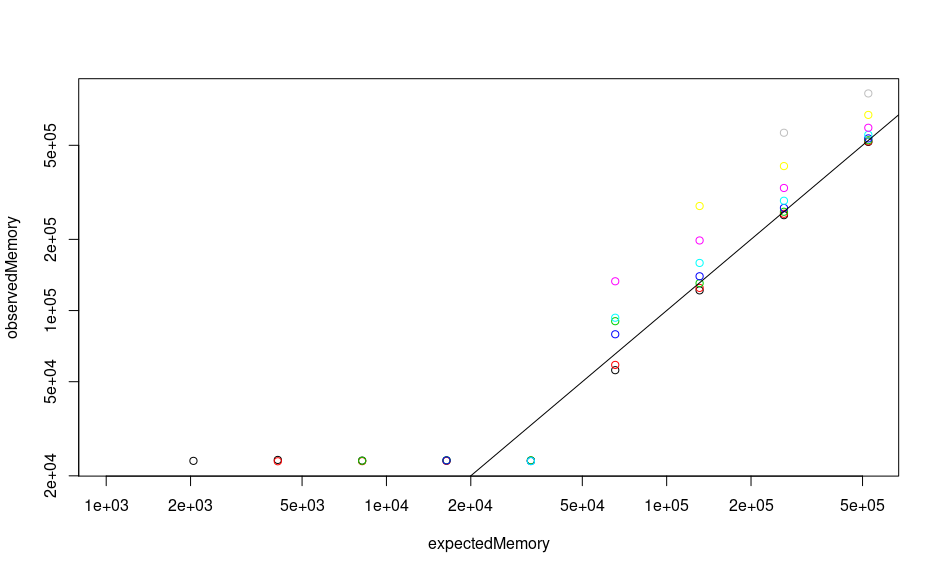
\includegraphics[width=\textwidth]{../proof_of_concept/comparison1.png}
  \caption{}
  \label{}
\end{figure}

\begin{figure}
  \centering
  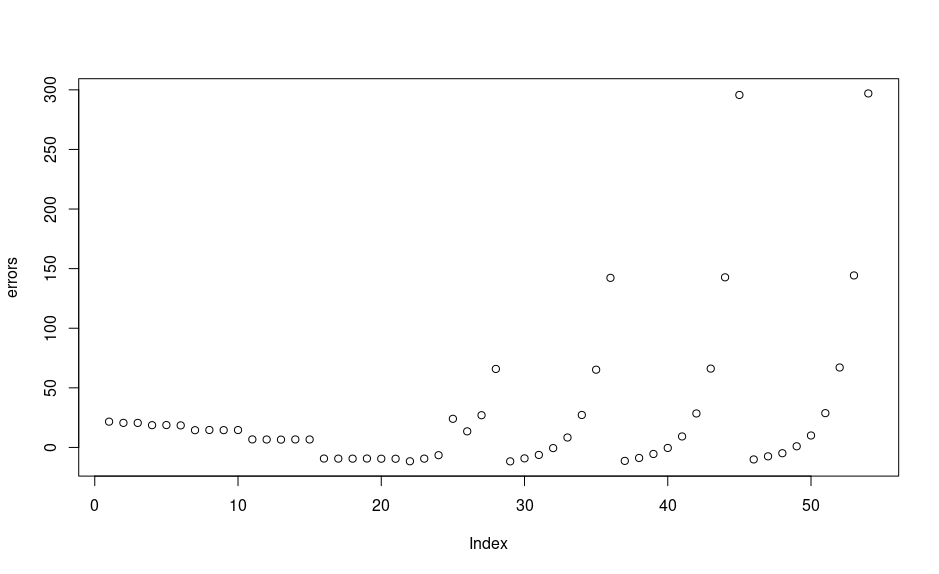
\includegraphics[width=\textwidth]{../proof_of_concept/comparison2.png}
  \caption{}
  \label{}
\end{figure}

\subsection{Adjusted Performance}

\begin{figure}
  \centering
  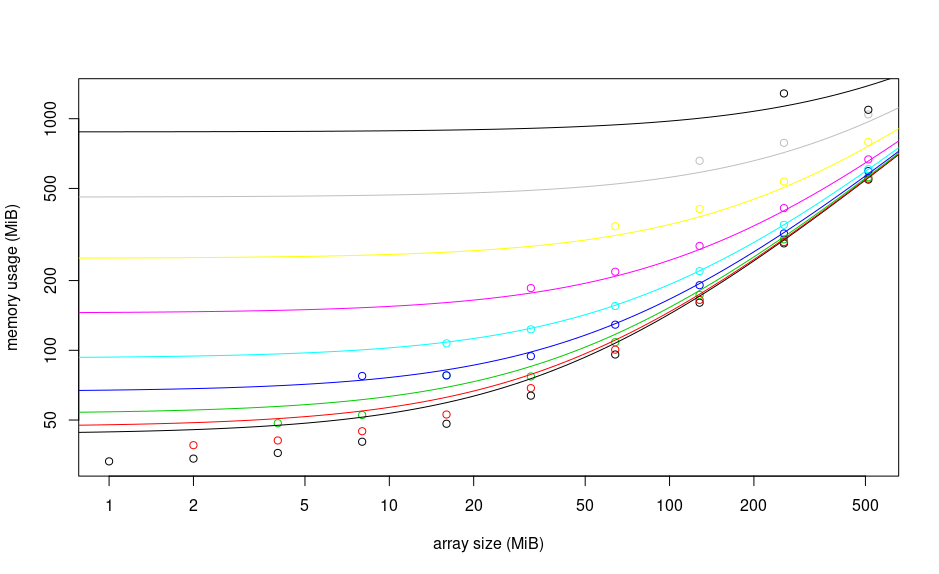
\includegraphics[width=\textwidth]{../proof_of_concept/prediction1.png}
  \caption{}
  \label{}
\end{figure}

\begin{figure}
  \centering
  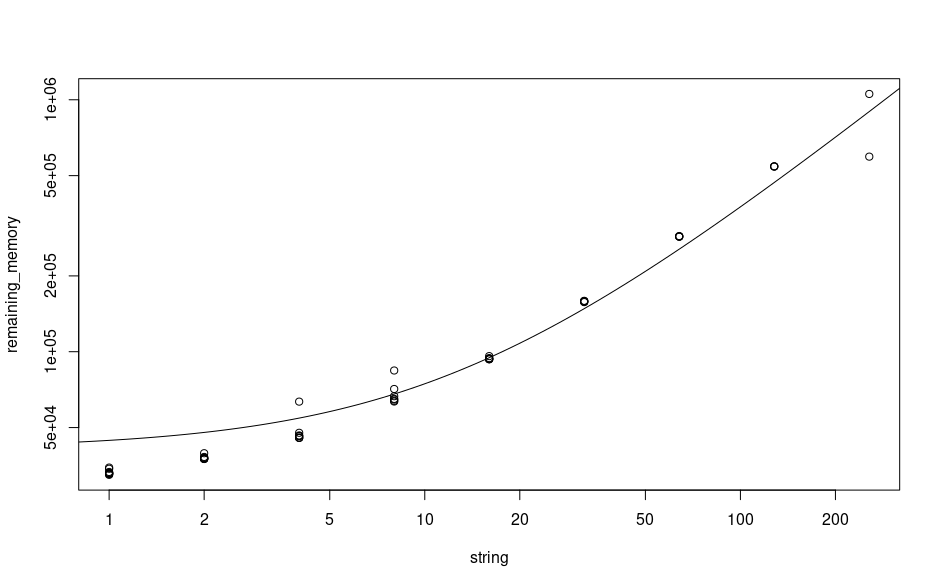
\includegraphics[width=\textwidth]{../proof_of_concept/prediction2.png}
  \caption{}
  \label{}
\end{figure}

\section{Experimental Results}
% TODO: a study that (visually) compares expected performance with Prometheus
% graphs for a range of (one-component) configurations

\section{Conclusion}

\end{document}